\documentclass[12pt, a4paper]{article}

\usepackage{fancyhdr}
\usepackage[left=4cm, right=4cm, top=4cm, bottom=4cm]{geometry}
\usepackage[utf8]{inputenc}
\usepackage[table]{xcolor}
\usepackage{hyperref}
\usepackage{amsmath}
\usepackage{enumitem}
\usepackage{graphicx}
\usepackage{booktabs}
\usepackage{subcaption}
\usepackage{xepersian}

\DeclareMathOperator*{\argmax}{argmax}
\DeclareMathOperator*{\argmin}{argmin}
\newcolumntype{L}{>{$}l<{$}} % math-mode version of "l" column type

\newcommand{\coursetitle}{شبکه‌های عصبی}
\newcommand{\doctitle}{تمرین دوم}
\newcommand{\name}{محمدرضا غفرانی}
\newcommand{\studentno}{400131076}
\newcommand{\todaydate}{\today}

\settextfont{Sahel}
\setlatintextfont{Times Newer Roman}

\pagestyle{fancy}
\lhead{\textbf{\doctitle}}
\chead{\name}
\rhead{\todaydate}

\begin{document}

\begin{flushleft}
    \name \\
    \studentno \\
    \todaydate
\end{flushleft}

\begin{center}
    \huge
    \textbf{\coursetitle}
    \break
    \large
    \doctitle
\end{center}

% suppress the fancy header on the first page only
\thispagestyle{plain}

\section*{سوال یک}

بر طبق توضیحات موجود در فایل پیوست دادگان، ویژگی‌های \lr{A1}, \lr{A2}, \lr{A4}, \lr{A5}, \lr{A6}, \lr{A7} و
\lr{A14} دارای مقادیر گمشده هستند. بنا به همین فایل پیوست، به جز ویژگی‌های \lr{A2} و \lr{A14} باقی ویژگی‌ها
کیفی هستند. از آن جا که توضیحی در بابت ویژگی‌های مختلف و معنی آن‌ها داده نشده است، بنابراین برای پر کردن
مقادیر گمشده در داده‌های کیفی از مد داده‌های معلوم و برای داده‌های کمی از میانگین استفاده می‌کنیم. البته برای داده‌های
ستون \lr{A14} استثنا قائل شده و مقادیر این ستون را علی‌رغم توضیحات فایل پیوست مجموعه دادگان، به صورت کیفی
در نظر می‌گیریم. علت انجام این کار وجود دو صفر در سمت چپ بیشتر اعداد این ستون است. اگر مقادیر این ستون
واقعا به صورت کمی بودند وجود این صفر‌ها پشت اعداد قابل توجیه نیست. همچنین در ستون برچسب‌های + و - را به
اعداد صفر و یک نگاشت می‌کنیم. باقی پیش‌پردازش‌ها در هنگام ورودی داده به شبکه صورت می‌گیرد. این پیش‌پردازش‌ها به
طور خلاصه به شرح زیر است.

\begin{enumerate}
    \item تبدیل ستون‌های کمی به بازه $[0,1]$ با استفاده از فرمول:
    $$\frac{\text{\lr{input}} - \text{\lr{mean}}}{\sqrt{\text{\lr{var}}}}$$
    \item کد‌گذاری مقادیر کیفی به صورت \lr{one hot}.
\end{enumerate}

\clearpage

\section*{سوال دو}

با توجه به شکل \ref{linear} که نمودار توزیع داده‌ها به صورت دو به دو رسم شده است، داده‌ها به صورت خطی قابل دسته‌بندی نیستند.
اما تنها با استفاده از این روش نمی‌توان در مورد جداپذیر خطی بودن نظر داد. در قدم بعدی از مدل
\lr{Linear Discriminant Analysis} استفاده می‌کنیم. این مدل سعی می‌کند داده‌ها را به بهترین شکل
از هم جدا کند. دسته‌بندی انجام شده توسط این دسته‌بند در شکل \ref{lda} دیده می‌شود. در این شکل محور
\lr{y} برچسب نسبت داده شده به داده و محور x تصویر داده‌ها روی محوری است که به بهترین نحو می‌توانسته است
داده‌ها را از هم جدا کند.

\begin{figure}[h]
    \centering
    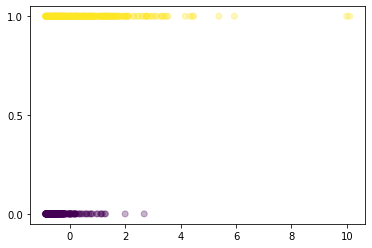
\includegraphics[width=0.4\linewidth]{images/lda.png}
    \caption{بررسی جداپذیر خطی بودن داده‌ها با استفاده از \lr{LDA}}
    \label{lda}
\end{figure}

در نهایت برای اطمینان از مدل \lr{SVM} با حاشیه سخت استفاده می‌کنیم.
بدین صورت که ابتدا مدل \lr{SVM} با کرنل خطی را بر روی داده‌های پیوسته آموزش داده و در قدم بعدی
سعی می‌کنیم این داده‌ها را با استفاده از مدل آموزش دیده جدا کنیم. با انجام این روش صحت دسته‌بندی مجدد
داده‌ها برابر ۳۰ درصد می‌شود. بنابراین نتیجه داده‌ها جداپذیر خطی نیستند چرا که اگر به صورت خطی جداپذیر
بودند با استفاده از این مدل باید به دقت نزدیک به ۱۰۰ دست می‌یافتیم.

\begin{figure}[h]
    \centering
    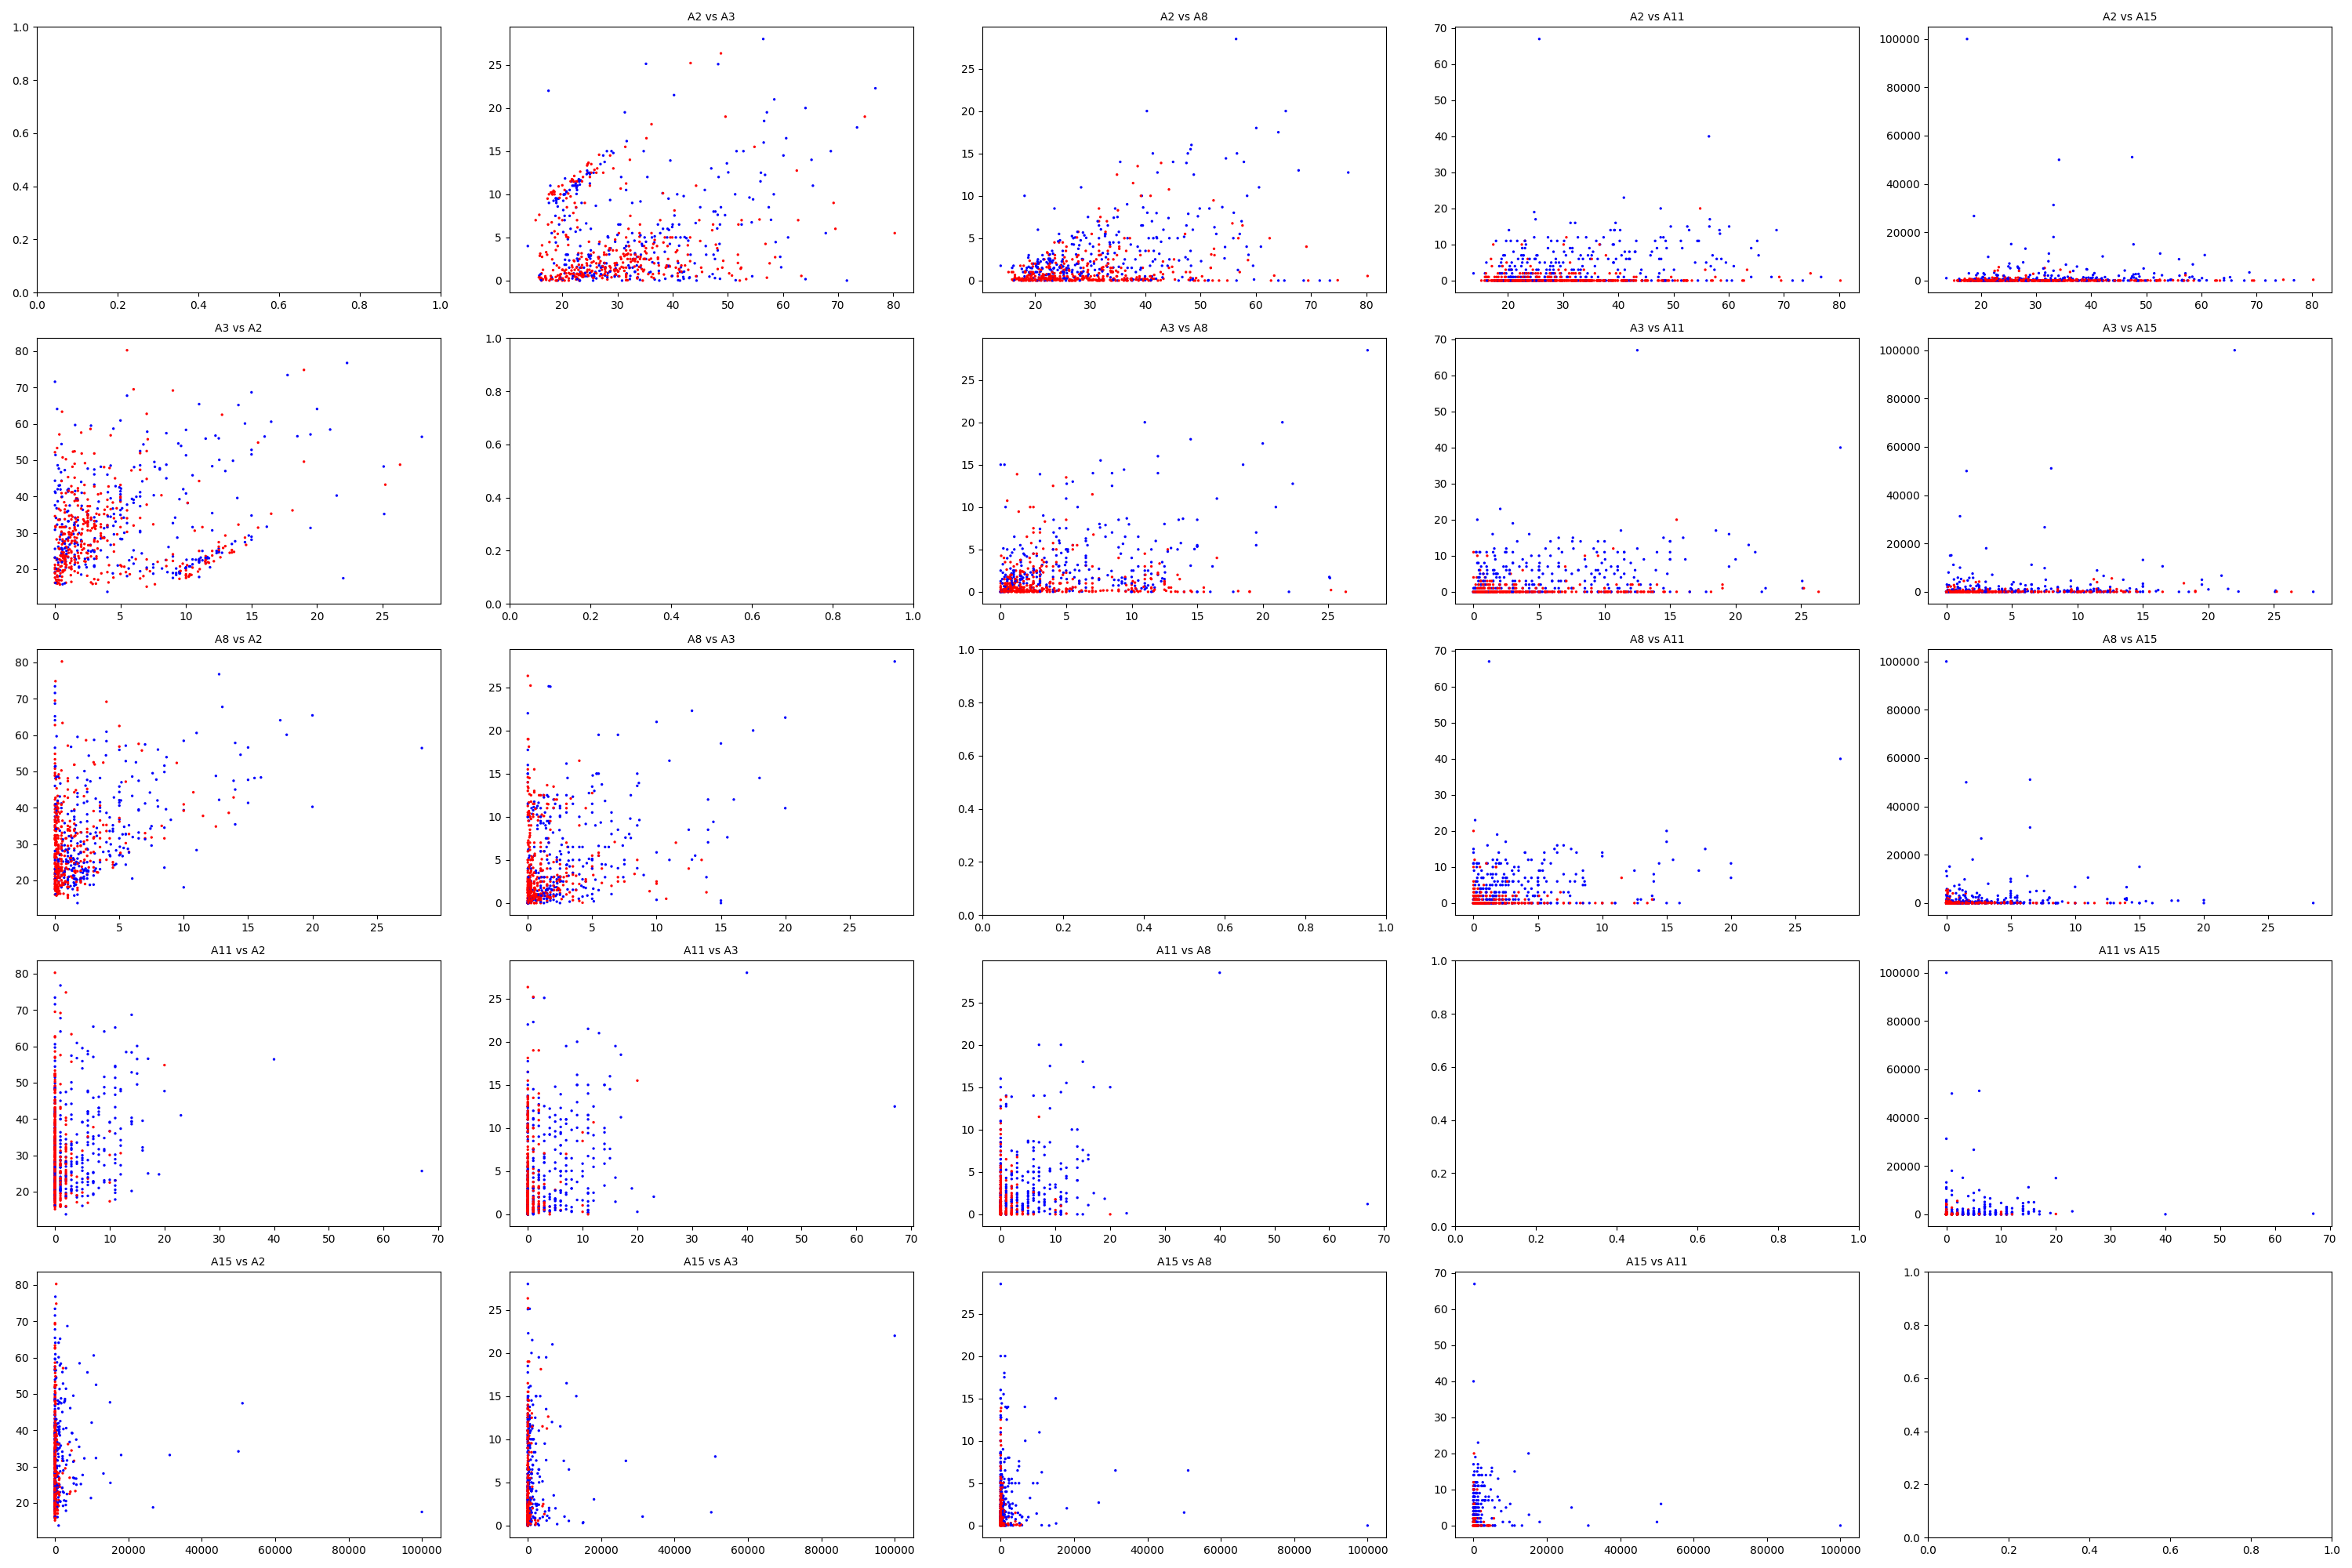
\includegraphics[width=0.8\linewidth]{images/linear.png}
    \caption{بررسی جداپذیر خطی بودن داده‌ها}
    \label{linear}
\end{figure}

\clearpage

\section*{سوال سه}

گراف این شبکه در شکل \ref{model} دیده می‌شود. همان‌طور که در این شکل قابل مشاهده است،
برای ویژگی‌های پیوسته یک لایه نرمال‌سازی در نظر گرفته شده است تا تمامی مقادیر به بازه‌های
$(0,1)$ نگاشت شود. برای ویژگی‌های گسسته نیز دو لایه پیش‌پردازش در نظر گرفته شده است:
یک لایه \lr{StringLookup} که وظیفه تهیه مجموعه لغات را به عهده دارد و یک لایه
\lr{CategoricalEncoding} که وظیفه تبدیل مقادیر عددی تولید شده به وسیله لایه \lr{StringLookup}
به بردار‌های \lr{One Hot} را انجام می‌دهد. در ادامه تمامی بردار‌های تولید برای تمامی ویژگی‌ها
به هم ملحق شده و به شبکه عصبی چندلایه پرسپترونی برای پردازش داده می‌شود. این شبکه عصبی
علاوه بر لایه‌های ورودی و خروجی، دو لایه پنهان نیز دارد. لایه پنهان اول ۳۲ و لایه پنهان دوم
۱۶ پرسپترون دارد. از تابع \lr{sigmoid} به عنوان تابع فعالیت این نورون‌ها استفاده شده است.
از بهینه‌ساز \lr{Adam} برای بهینه‌سازی مدل و از تابع خطای \lr{Binary Cross Entropy} برای ارزیابی
عملکرد این مدل استفاده شده است.

\begin{figure}[h]
    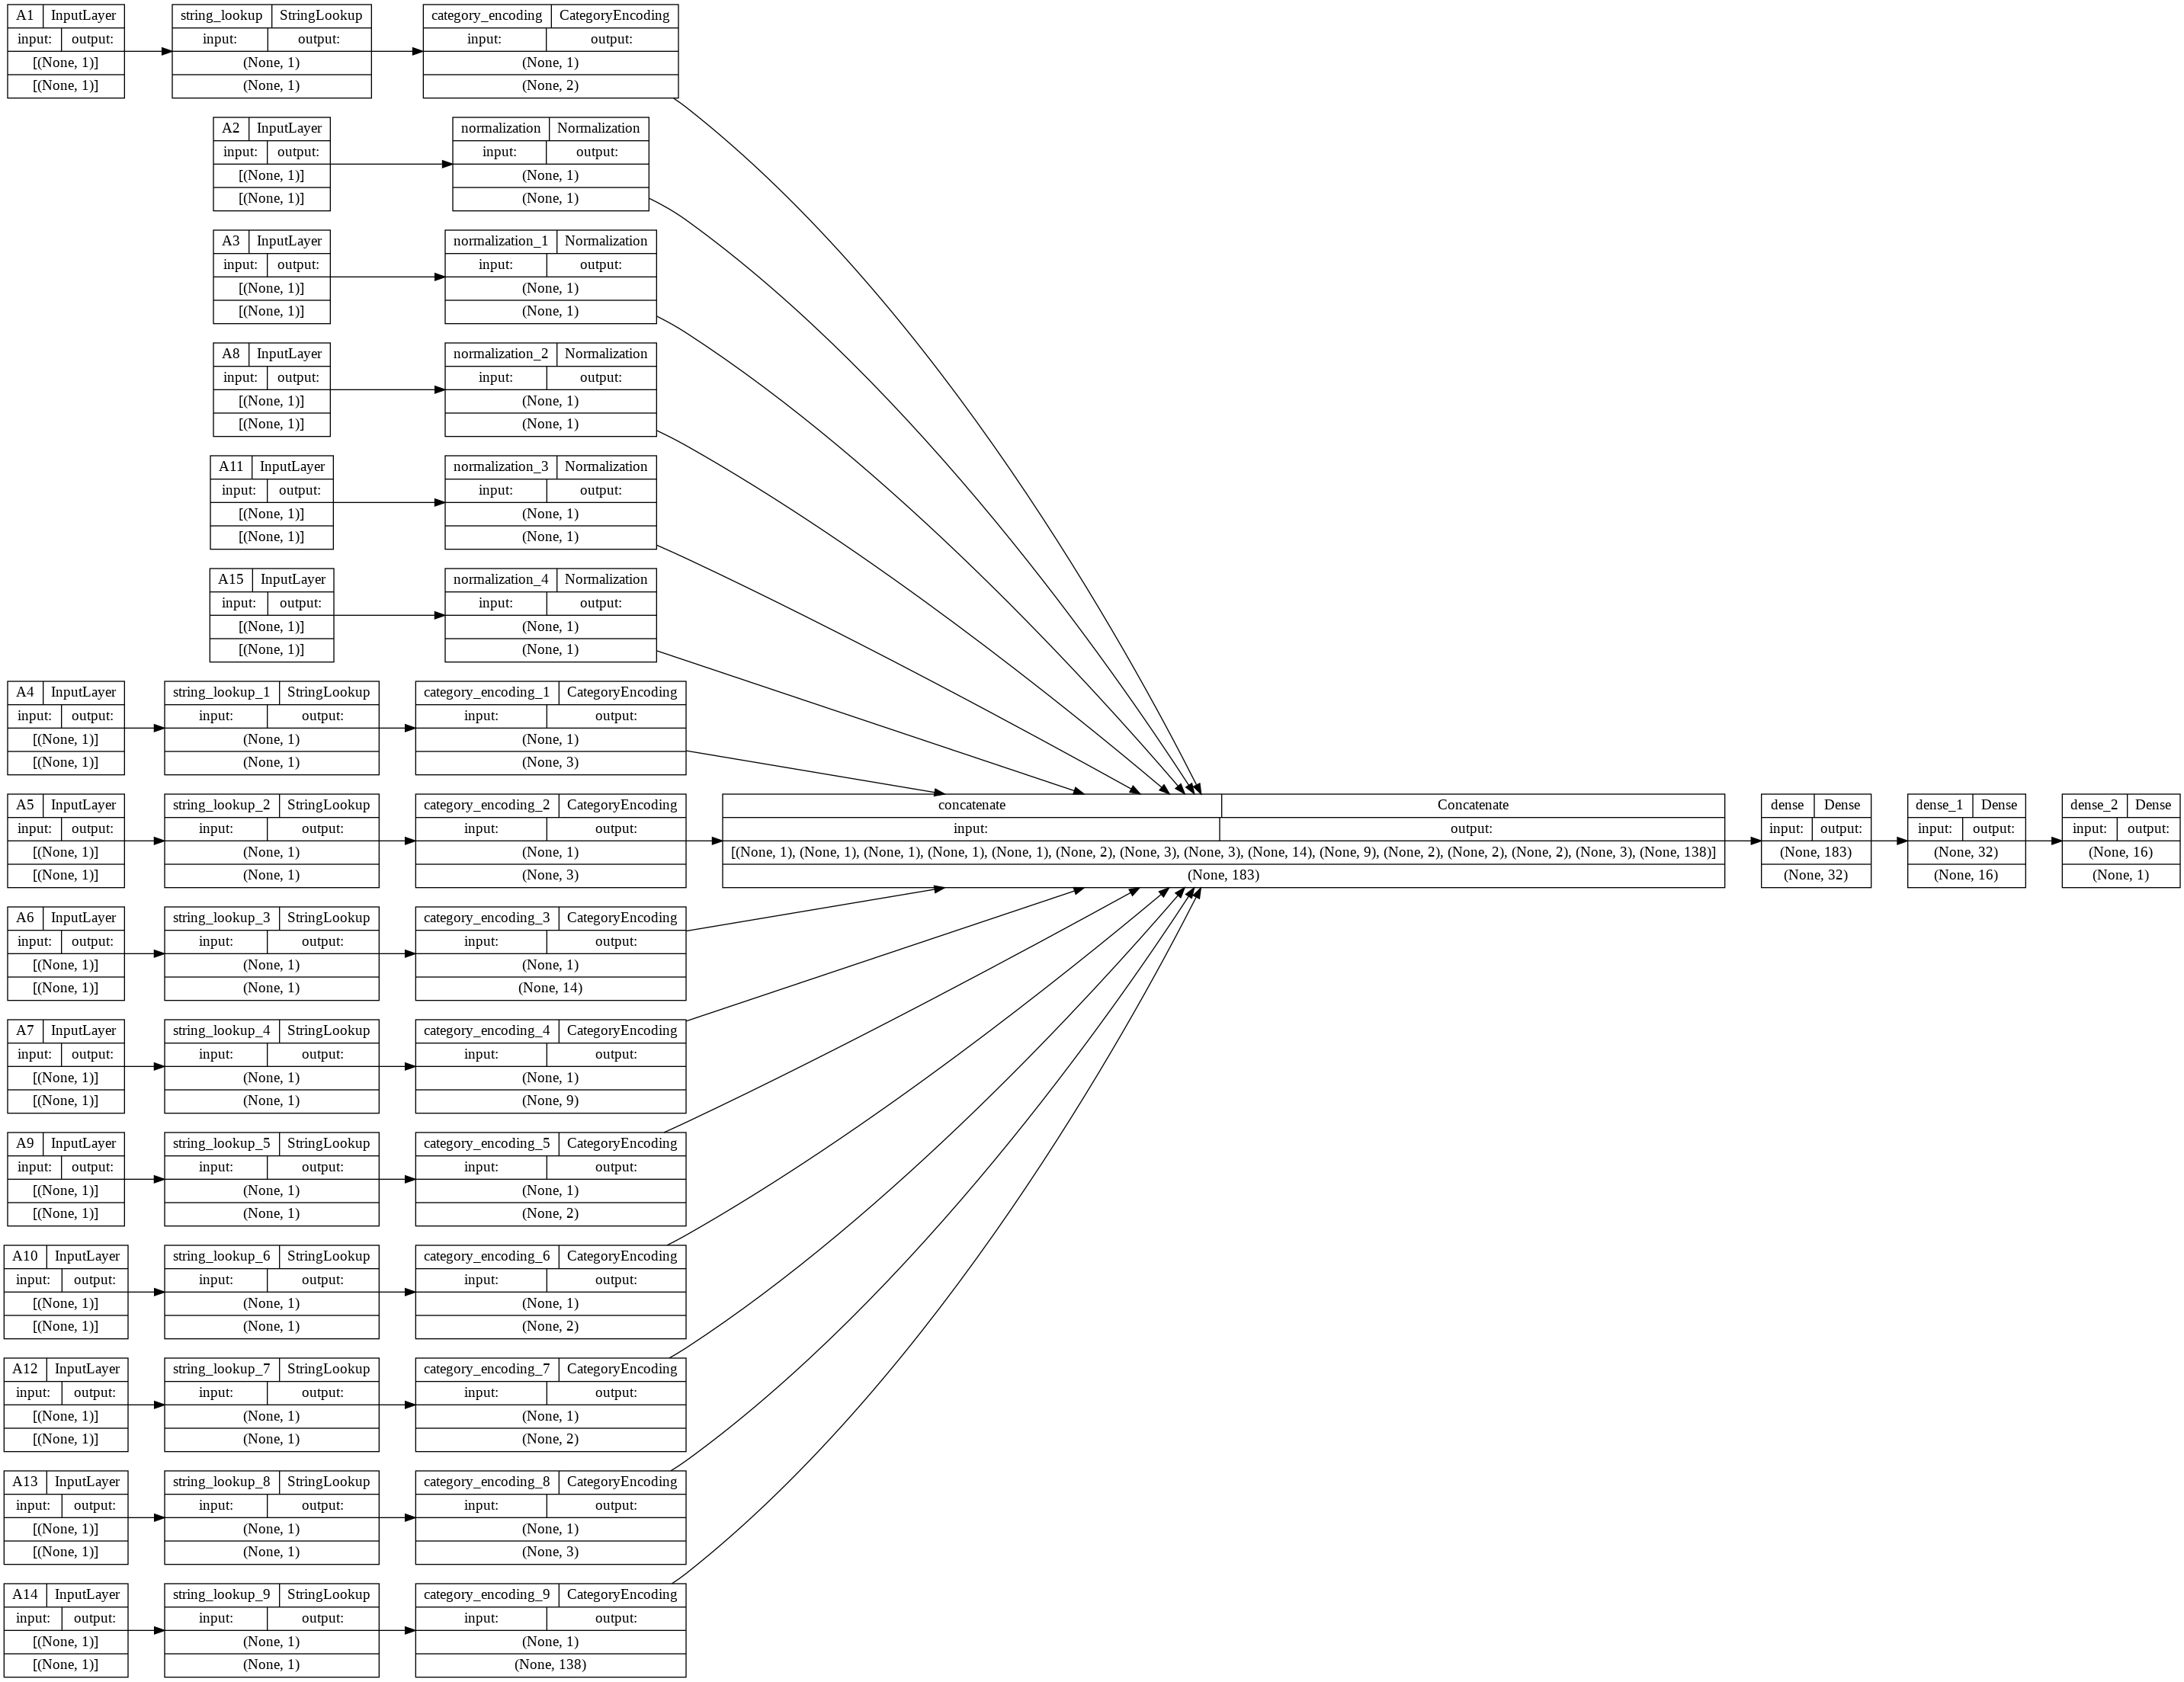
\includegraphics[width=\linewidth]{images/model.png}
    \caption{گراف شبکه عصبی سوال سوم}
    \label{model}
\end{figure}

اگر شبکه حاصل شده را با استفاده از \lr{tensor board} مورد بررسی قرار دهیم، شکل مدل به صورت زیر حاصل
می‌شود.(شکل \ref{tensorboard_model}) همچنین با دوبار کلیک کردن بر روی مدل و لایه‌های آن می‌توان اطلاعات دقیق‌تری
از مدل به دست آورد.

\begin{figure}[h]
    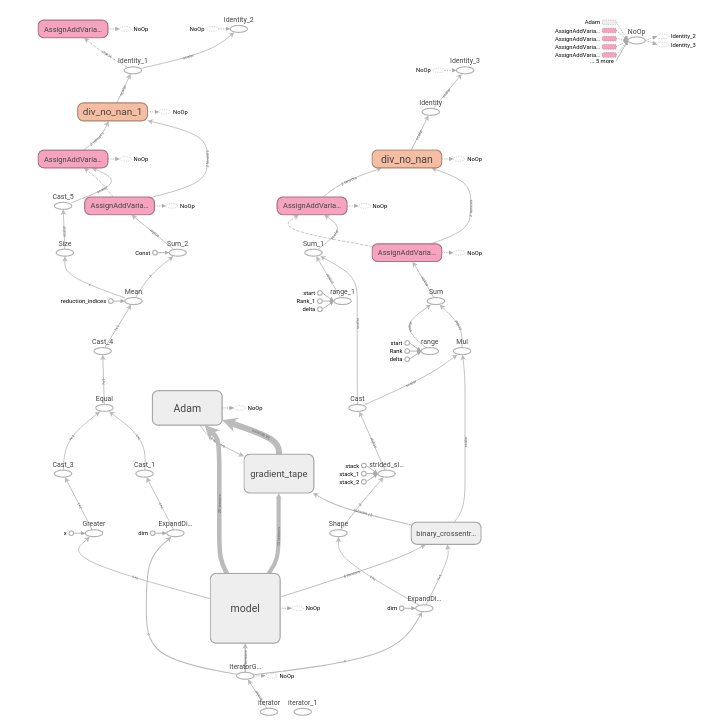
\includegraphics[width=\linewidth]{images/tensorboard_model.png}
    \caption{گراف شبکه عصبی سوال سوم با استفاده از ابزار \lr{tensorboard}}
    \label{tensorboard_model}
\end{figure}

\begin{figure}[h]
    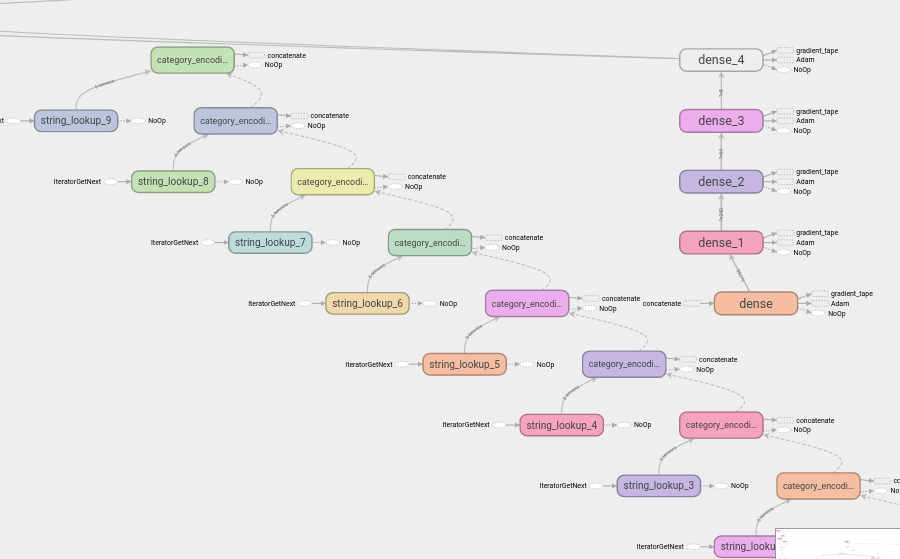
\includegraphics[width=\linewidth]{images/details.png}
    \caption{جزئیات مدل سوال سوم}
    \label{details}
\end{figure}


\clearpage

\section*{سوال چهار}

در این سوال شبکه استفاده شده، مشخصات شبکه استفاده شده در سوال سه را دارد. تنها قسمتی که در این سوال
دستخوش تغییر می‌شود تعداد لایه‌های میانی و تعداد نورون‌های موجود در این لایه‌های میانی است.

در جدول \ref{2layer_mlp} آزمون خطاهای انجام شده برای یافتن بهترین تعداد پرسپترون در حالتی که
دو لایه مخفی وجود دارد، آورده شده است. رویکرد ما برای انتخاب تعداد نورون‌های هر لایه بررسی هر یک از اعداد موجود در لیست
$[16,32,64,100,128]$ برای هر یک از لایه‌های میانی است. بر طبق مشاهدات انجام شده،
شبکه‌عصبی پرسپترونی دو لایه در حالتی که لایه اول تعداد پرسپترون بیشتری دارد، بهتر عمل می‌کند.
بعلاوه بر طبق همین مشاهدات، در حالتی که تعداد
پرسپترون‌های لایه اول برابر ۸۰ و تعداد پرسپترون‌های لایه دوم برابر ۱۶ است بهترین عملکرد را دارد.

\begin{table}[h]
    \centering
    \caption{\rl{آزمون‌خطاهای انجام شده برای یافتن پارامتر‌ها در حالت وجود دو لایه پنهان}}
    \label{2layer_mlp}
    \begin{tabular}{L|L|L|L}
        \text{لایه ۱} & \text{لایه ۲} & \text{صحت داده آموزشی} & \text{صحت داده ارزیابی} \\
        \hline
        16 & 16 & 0.5622 & 0.6714 \\
        32 & 16 & 0.6286 & 0.7571 \\
        64 & 16 & 0.7842 & 0.8286 \\
        80 & 16 & 0.7759 & 0.8286 \\
        100& 16 & 0.7593 & 0.8571 \\
        128& 16 & 0.7241 & 0.8000 \\
        16 & 32 & 0.5830 & 0.7143 \\
        16 & 64 & 0.5705 & 0.7000 \\
        16 & 80 & 0.6058 & 0.7429 \\
        16 & 100& 0.5913 & 0.7429 \\
        16 & 128& 0.5788 & 0.7429 \\
    \end{tabular}
\end{table}

\clearpage

در این سوال، در حالتی که شبکه عصبی چندلایه پرسپترونی سه لایه دارد، نسبت به زمانی که دو لایه پنهان
دارد عملکرد بهتری را از خود نشان می‌دهد. جدول \ref{3layer_mlp} نشان‌دهنده آزمون‌خطاهای انجام شده در این حالت است.
برای یافتن بهترین تعداد پارامتر برای هر لایه، به روش حریصانه عمل می‌کنیم. ابتدا تعداد پرسپترون‌های موجود
در لایه اول را تغییر داده و تعداد پرسپترونی که به ازای آن مدل نتایج بهتری می‌گیرد را پیدا می‌کنیم. سپس
به همین ترتیب بهترین تعداد پرسپترون را برای لایه دوم و سوم پیدا می‌کنیم. نتایج آزمون و خطاهای انجام شده
در جدول زیر دیده می‌شود. در این حالت نیز مطابق انتظار با افزایش نورون‌های لایه‌های میانی
رفته‌رفته عملکرد مدل، بهتر و بهتر شده است اما از یک نقطه به بعد به نظر می‌رسد که مدل دچار بیش‌برازش شده باشد،
چرا که نتایج مدل بر روی داده‌های ارزیابی ضعیف‌تر می‌شود. به همین دلیل آزمون‌‌‌وخطا را در حالت
وجود سه لایه میانی در همین حد نگه داشته و بیشتر ادامه نمی‌دهیم.

\begin{table}[h]
    \centering
    \caption{\rl{آزمون‌خطاهای انجام شده برای یافتن پارامتر‌ها در حالت وجود سه لایه پنهان}}
    \label{3layer_mlp}
    \begin{tabular}{L|L|L|L|L}
        \text{لایه ۱} & \text{لایه ۲} & \text{لایه ۳} & \text{صحت داده آموزشی} & \text{صحت داده ارزیابی} \\
        \hline
        64 & 32 & 16 & 0.6286 & 0.7714 \\
        80 & 32 & 16 & 0.7252 & 0.8286 \\
        100& 32 & 16 & 0.7510 & 0.8571 \\
        128& 32 & 16 & 0.7095 & 0.8429 \\
        100& 64 & 16 & 0.7593 & 0.8571 \\
        100& 80 & 16 & 0.8133 & 0.8714 \\
        100& 100& 16 & 0.8278 & 0.8857 \\
        100& 128& 16 & 0.8278 & 0.9143 \\
        100& 150& 16 & 0.8423 & 0.8857 \\
        100& 180& 16 & 0.7116 & 0.8286 \\
        100& 128& 32 & 0.8382 & 0.9000 \\
        100& 128& 64 & 0.7593 & 0.9000 \\
        100& 128& 80 & 0.8423 & 0.8857 \\
        100& 128& 80 & 0.8423 & 0.8714
    \end{tabular}
\end{table}

\clearpage

عملکرد مدل در حالت وجود ۴ لایه پنهان در جدول \ref{4layer_mlp} دیده می‌شود. با مقایسه نتایج این مدل
با حالت‌های قبلی مشخص می‌شود که عملکرد مدل چندان تغییر نکرده است. بهترین نتیجه این مدل صحت ۹۱ درصد
در داده‌های ارزیابی و صحت ۸۶ درصد در داده‌های آموزشی است. در حالت وجود ۳ لایه پنهان بهترین نتیجه صحت
۹۱ درصد در داده ارزیابی و صحت ۸۲ درصد در داده آموزشی بود. همان‌طور که مشاهده می‌شود اضافه کردن لایه‌های
جدید دیگر عملکرد مدل را آنچنان بهبود نداده است. اگر بخواهیم به نتایج موجود در این جدول دقیق‌تر نگاه کنیم، متوجه می‌شویم که در ابتدا
با اضافه کردن نورون‌های جدید به شبکه صحت مدل روی داده‌های آموزشی به یکباره از ۶۷ درصد به مقدار ۸۰ درصد
می‌رسد اما در ادامه با زیاد‌کردن تعداد پرسپترون‌ها تغییر شگرفی در نتایج عملکرد مدل دیده نمی‌شود.
بنابراین به نتایج به دست آمده اکتفا کرده و از بررسی حالت‌های جدید صرف‌نظر می‌کنیم.
در نهایت به نظر می‌رسد که مدل با ۴ لایه مخفی و تعداد نورون‌های موجود در هر لایه
150، ۲۴۰، ۶۴ و ۸ به بهترین نتیجه را داشته و در نتیجه همین مدل را در ادامه در نظر می‌گیریم.

\begin{table}[h]
    \centering
    \caption{\rl{آزمون‌خطاهای انجام شده برای یافتن پارامتر‌ها در حالت وجود چهار لایه پنهان}}
    \label{4layer_mlp}
    \begin{tabular}{L|L|L|L|L|L}
        \text{لایه ۱} & \text{لایه ۲} & \text{لایه ۳} & \text{لایه ۴} & \text{صحت داده آموزشی} & \text{صحت داده ارزیابی} \\
        \hline
        64 & 32 & 16 & 8 & 0.6743 & 0.8000 \\
        80 & 32 & 16 & 8 & 0.6971 & 0.8000 \\
        100 & 32 & 16 & 8 & 0.7697 & 0.8286 \\
        150 & 32 & 16 & 8 & 0.8071 & 0.8714 \\
        180 & 32 & 16 & 8 & 0.8008 & 0.8571 \\
        200 & 32 & 16 & 8 & 0.7261 & 0.8286 \\
        150 & 64 & 16 & 8 & 0.8133 & 0.8571 \\
        150 & 80 & 16 & 8 & 0.8361 & 0.9143 \\
        150 & 100 & 16 & 8 & 0.8216 & 0.9000 \\
        150 & 128 & 16 & 8 & 0.8423 & 0.9000 \\
        150 & 150 & 16 & 8 & 0.8340 & 0.8857 \\
        150 & 180 & 16 & 8 & 0.8423 & 0.9000 \\
        150 & 240 & 16 & 8 & 0.8568 & 0.9143 \\
        150 & 280 & 16 & 8 & 0.8567 & 0.8857 \\
        150 & 320 & 16 & 8 & 0.8568 & 0.8857 \\
        150 & 240 & 32 & 8 & 0.8340 & 0.9000 \\
        150 & 240 & 64 & 8 & 0.8610 & 0.9143 \\
        150 & 240 & 80 & 8 & 0.8568 & 0.9000 \\
        150 & 240 & 100 & 8 & 0.8651 & 0.9143 \\
        150 & 240 & 128 & 8 & 0.8568 & 0.9000 \\
        150 & 240 & 128 & 32 & 0.8506 & 0.9143 \\
        150 & 240 & 128 & 80 & 0.8568 & 0.9000 \\
    \end{tabular}
\end{table}

\clearpage

\section*{سوال پنجم}

در این حالت مشابه اکثر کار‌های یادگیری ماشین باید تعداد پارامتر‌های مدل را آنقدر زیاد کنیم تا
مدل تلاش کند داده‌های آموزشی را حفظ کند. برای رسیدن به این حالت هم تعداد لایه‌ها و
هم تعداد پرسپترون موجود در هر لایه را زیاد می‌کنیم. ما در این جا تعداد لایه‌های پنهان مدل را ۶ و تعداد
پرسپترون هر لایه را ۵۰۰ در نظر می‌گیریم. همچنین مدل را در ۱۰۰ گام آموزش می‌دهیم تا مدل فرصت بیش‌برازش داشته باشد.

بعد از آموزش این مدل صحت در داده آموزشی، تست و ارزیابی تفاوت فاحشی با هم ندارد. صحت
در داده‌ آموزشی، ارزیابی و تست به ترتیب برابر ۹۶، ۸۸ و ۸۲ درصد می‌شود. اما معیار \lr{loss}
در داده‌های آموزشی، ارزیابی و تست به ترتیب برابر $0.14$، $0.44$ و $0.58$ می‌شود. همان‌طور
که مشاهده می‌شود، اختلاف \lr{loss}ها در داده‌ آموزش با داده‌های ارزیابی و تست زیاد است.
که این نشانگر بیش‌برازش است. در ادامه نمودار برای داده‌های آموزش و ارزیابی مشاهده می‌شود.
همان‌طور که مشاهده می‌شود در ابتدا داده‌های آموزشی به یک صحت مشخص می‌رسد اما بعد از آن شاهد
پدیده بیش‌برازش هستیم.

\begin{figure}[h]
    \centering
    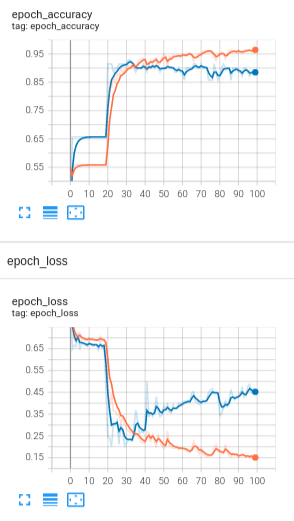
\includegraphics[scale=0.5]{images/graph.png}
    \caption{نمودار تغییرات صحت و \lr{loss} در گام‌های مختلف برای داده‌های ارزیابی و آموزش}
    \label{loss}
\end{figure}

\clearpage

\section*{سوال ششم}

برای این کار همانند روند انجام شده در سوال ۲ پیش می‌رویم و سعی می‌کنیم پارامتر‌های شبکه عصبی را
طوری تغییر می‌دهیم تا شبکه عصبی به نتایج خوبی هم بر روی داده‌های آموزشی و هم بر روی داده‌ی ارزیابی
برسد. در نهایت نتایج حاصل از عملکرد شبکه بر روی داده‌های آموزشی و ارزیابی را با داده‌های تست
مقایسه می‌کنیم. اگر تفاوت فاحشی بین این نتایج وجود نداشته باشد، این به این معنی است که مدل تا
حد زیادی \lr{General} شده و قابلیت تعمیم‌پذیری دارد. برای این کار از بهترین مدلی که در سوال ۴ یافتیم
استفاده می‌کنیم. این مدل دارای ۴ لایه پنهان بوده و در هر لایه ۱۵۰، ۲۴۰، ۶۴ و ۸ نورون دارد.
این مدل را به تعداد ۱۰۰ گام آموزش می‌دهیم. برای جلوگیری از بیش‌برازش احتمالی از یک \lr{callback}
از نوع \lr{Early Stopping} نیز کمک می‌گیریم. در نهایت نتایج روی داده‌های آموزش و ارزیابی به شکل
\ref{general_model_results} حاصل می‌شود. همان‌طور که مشاهده می‌شود خطا و صحت بر روی داده‌های آموزشی و تست
با نرخ یکنواختی کاهش داشته است. معیار \lr{loss} که تاثیر زیادی در تعمیم مدل دارد نیز به نحو
مناسبی هم در داده آموزش و هم در داده ارزیابی کاهش یافته و به مقدار $0.2$ رسیده است.

\begin{figure}[h]
    \begin{subfigure}{0.45\linewidth}
        \centering
        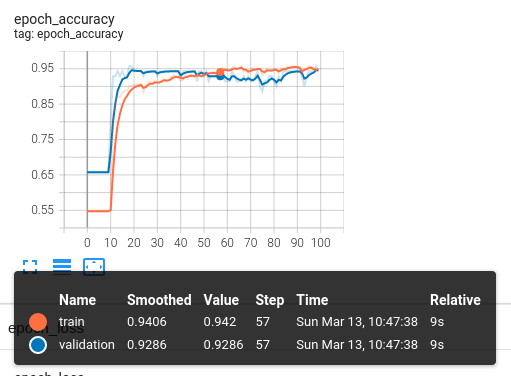
\includegraphics[width=\linewidth]{images/q6_acc.png}
    \end{subfigure}
    \begin{subfigure}{0.45\linewidth}
        \centering
        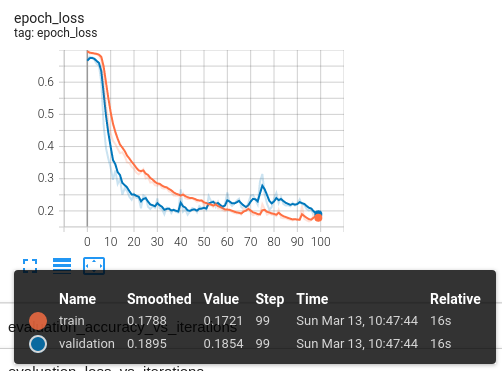
\includegraphics[width=\linewidth]{images/q6_loss.png}
    \end{subfigure}
    \caption{نمودار \lr{loss} و صحت در داده‌های آموزشی و ارزیابی}
    \label{general_model_results}
\end{figure}

برای اطمینان از عملکرد مدل از تکنیک \lr{kfold cross validation} نیز استفاده می‌کنیم.
همان‌طور که می‌دانید، در این روش داده‌های آموزشی به $k$ بخش تقسیم شده و هر بار با $k-1$ بخش آموزش دیده و با
بخش $k$ام تست می‌شود. اگر میانگین نتایج این تکنیک خوب باشد، بدین معنی است که مدل عملکرد مناسبی دارد.
با پیاده‌سازی روش \lr{k-fold cross validation}، میانگین صحت مدل برابر 84 درصد می‌شود که نتیجه قابل قبولی است.

\end{document}